\documentclass[11pt]{beamer}
\usetheme{Singapore}

\usepackage[utf8]{inputenc}
\usepackage[T1]{fontenc}
\usepackage{soul}
\usepackage{graphicx}


\graphicspath{{../../Figures/}}

\def\et{{\it et al.}}


\author{Cody Glickman \\ CPBS Update Talk}

\title{Metagenomic Exploration the Sequel: \\ Development of novel tools for viral and bacterial sequence analysis}

%\subtitle{}
%\logo{}

\date{ 
\includegraphics[height=2cm, width=2cm]{lablogo.png} \\ Jan 29th, 2018}
%\subject{}
\setbeamercovered{transparent}
\setbeamertemplate{navigation symbols}{}
\setbeamertemplate{theorems}[numbered]

\begin{document}
	\maketitle
	\begin{frame}{Research Update}
	\begin{block}{\alert{Clinical NTM Gene Databases}}
	Submitted ...
	https://mra.asm.org/latest 
	\end{block}
	
	\begin{block}{\alert{Duobiome: 18S/16S Parallel Analysis}}
	In progress
	\end{block}
	
	\begin{block}{\alert{Hybrid Viral Contig Prediction}}
	In progress
	\end{block}
	
	\begin{block}{\alert{Virulence Factors in Bacteriophages}}
	Submitted ...
	\end{block}
	\end{frame}
	
	\begin{frame}{Progress of Other Projects}
	\begin{block}{Asthma Environmental Microbiome}
	Submitted abstract to ATS
	\end{block}
	
	\begin{block}{Building Up Domains: Lysogenic Host Discovery}
	Incorporated into large collaborative NCBI initative
	\end{block}
	
	\begin{block}{Genomic Retrieval and Blast Database Creation}
	Accepted Poster ISME 2017
	\end{block}
	
	\begin{block}{Hawaiian Soil Chemistry and Culture}
	Submitted ...
	\end{block}
	

	\end{frame}
	%-----------------------------------------------------------
\section{}

	\begin{frame}{Nontuberculous Mycobacterial (NTM) Infections}
		\begin{block}{Number of Cases}
		The number of NTM cases is estimated over 100K
		\end{block}
		
		\begin{block}{Increasing Case}
		The rate of cases is estimated to grow at 8\% every year
		\end{block}
		
		
		\begin{block}{Populations at risk of developing NTM}
		\begin{itemize}
		\item Immunocompromised individuals 
		\item Patients with lung damage or malfunction 
		\item Residents of warm costal areas especially Hawaii
		%\item The Elderly 
		\end{itemize}
		\end{block} 
		
		\begin{block}
		
		\end{block}
	\vspace{-1cm}
	\tiny{Strollo SE, et al. Ann Am Thorac Soc. 2015 \\
	Adjemian J, et al. Am J Respir Crit Care Med. 2012}
	
	\end{frame}
	%----------------------------------------------------------
	\begin{frame}{Laboratory Research Methods}
	\begin{block}{Conditions for NTM Environmental Growth}
	Identifying important characteristics for NTM growth 
	\end{block}
	
	\begin{block}{Environmental Microbiome}
	Developing methods to characterize home environments
	\end{block}
	
	\begin{block}{Clinical NTM}
	\begin{itemize}
	\item 90\% of NTM cultures are from respiratory samples
	\item Identifying potential person-to-person transmission
	\end{itemize}
	\end{block}
	
	\tiny{O'Brien, R., et al. American Review of Respiratory Disease 1987}

	
	\end{frame}
	
	%-----------------------------------------------------------
	\begin{frame}{Viral Focus}
	
	\begin{block}{Bacteriophages (Phages)}
	Phages are DNA viruses that infect prokaryotes
	\end{block}
	
	\begin{block}{Phage Diversity}
	Investigating how phage abundance and diversity affect susceptibility to NTM lung infection
	\end{block}
	
	\begin{block}{Phage Vectors}
	Researching how phages act as carriers of bacterial genes within clinical NTM infections
	\end{block}
	
	\end{frame}
	%-----------------------------------------------------------
	\begin{frame}{Molecular Methods to Study Phages}
	\begin{columns}
	\column{0.5\textwidth}
	\begin{block}{Difficulties of phage study}
	\begin{itemize}
		\item Lack of universal marker gene
		\item Sequence heterogeneity 
		\item Misclassification in databases
	\end{itemize}
	\end{block}
		
		
	\begin{block}{Phage Isolation Methods}
	\begin{itemize}
		\item Biological filtration
		\item In silico methods
	\end{itemize}
	\end{block}
	
	\column{0.5\textwidth}
	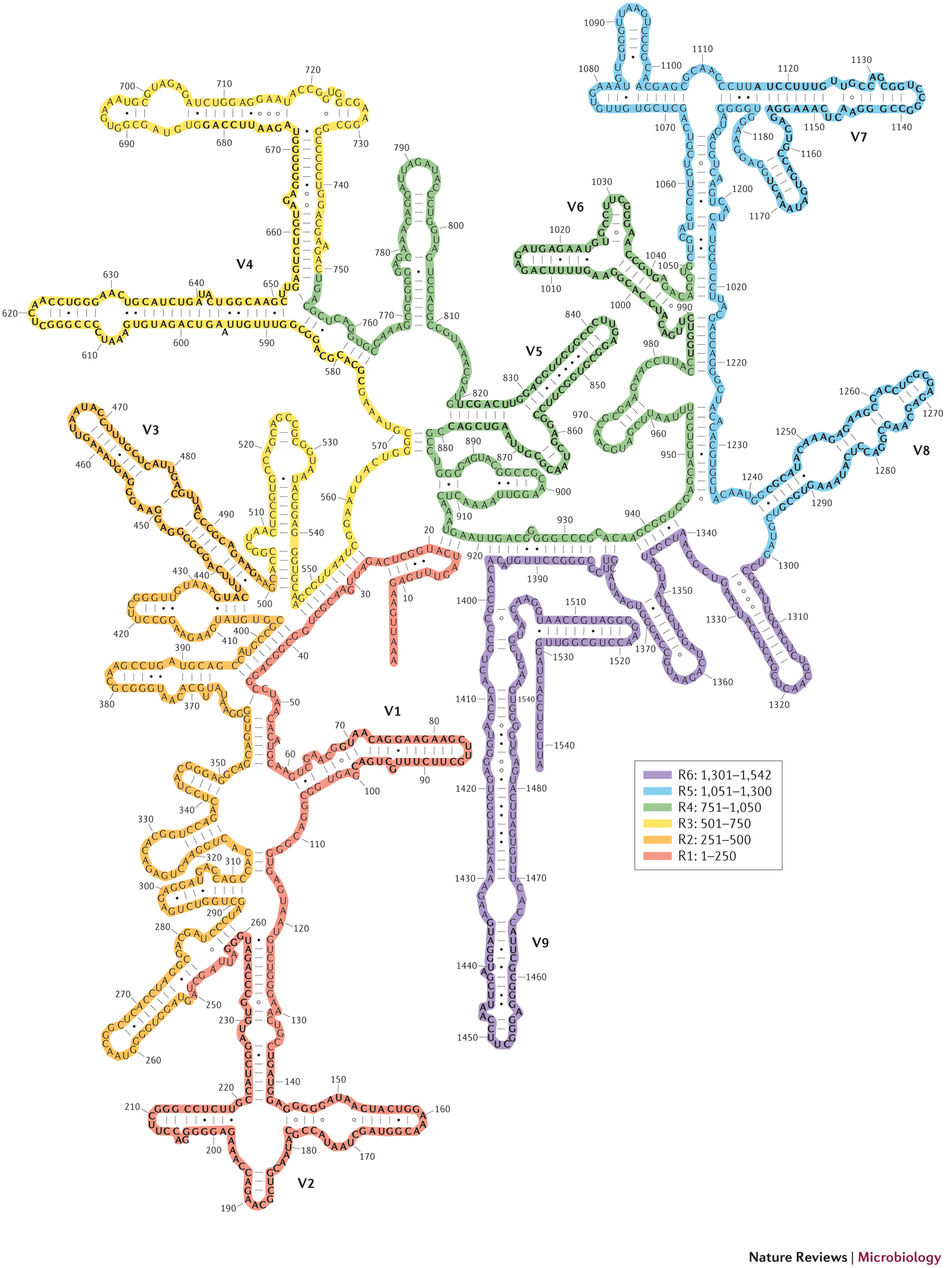
\includegraphics[height=5.5cm, width=5cm]{ribosome.jpg} \\
	\tiny{Yarza, P., et al. Nature Reviews Microbiology 2014}
	\end{columns}
		
	
	\end{frame}

	%-----------------------------------------------------------
	\begin{frame}{Objective}
	\center
	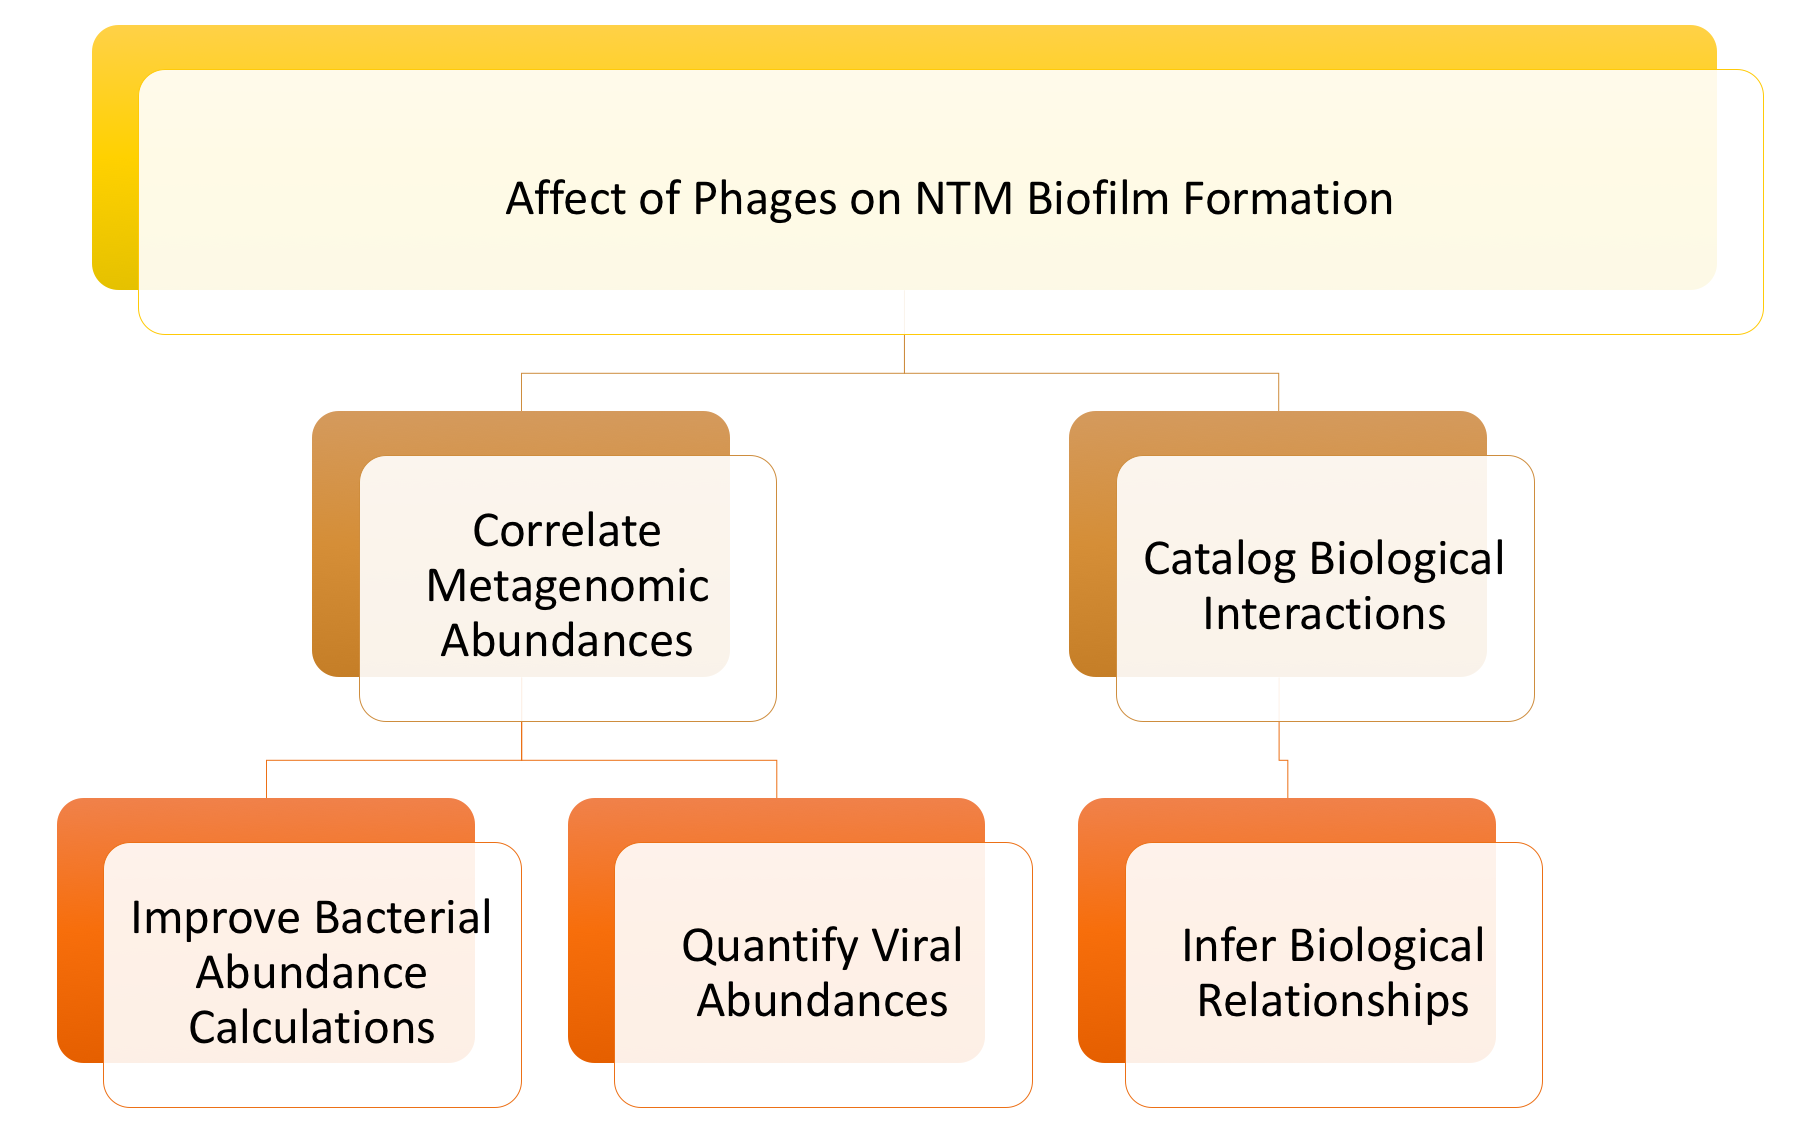
\includegraphics[height=6cm, width=9cm]{objective.png}
	
	\end{frame}

%-----------------------------------------------------------
	
\section{Clinical NTM Gene Databases}
\subsection{}
	\begin{frame}{Species Identification of NTM at NJH}

	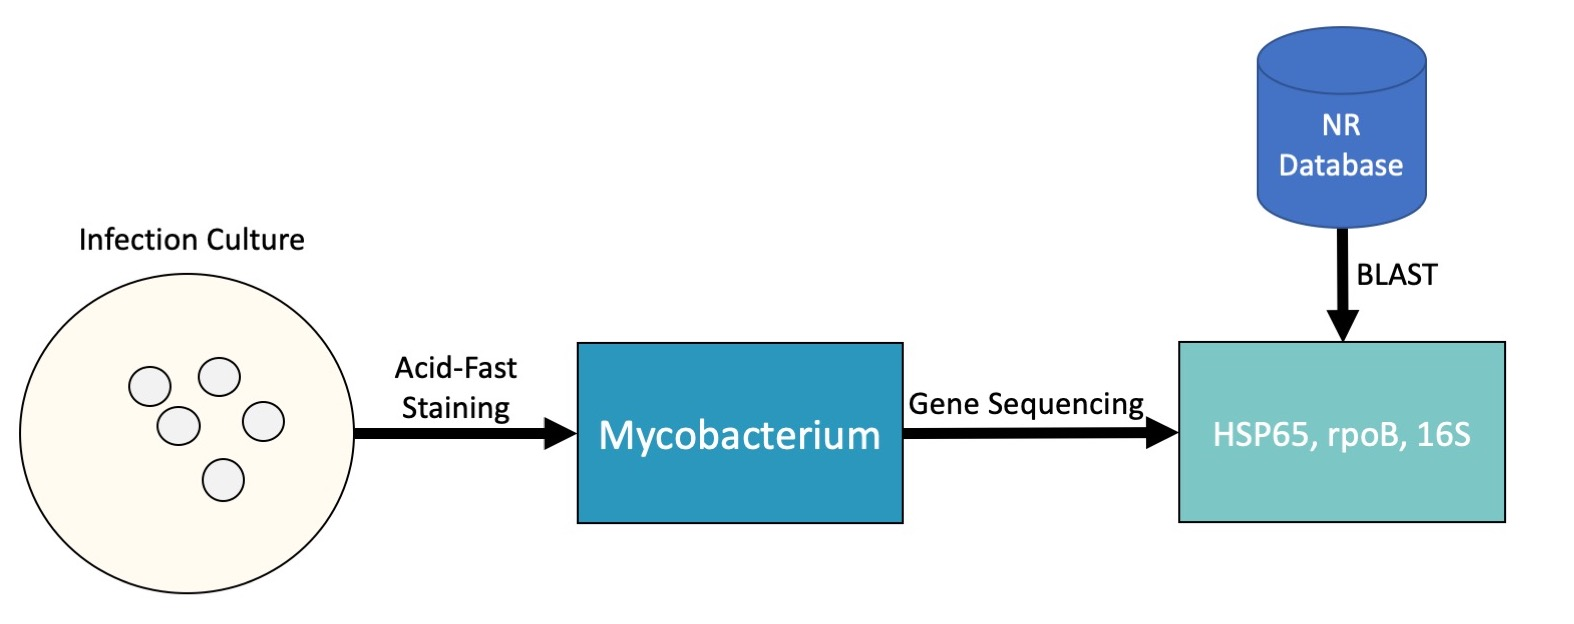
\includegraphics[height=5cm, width=11cm]{CPBS_11_18/NJH_Protocol.jpg}
	
	\end{frame}
	%-----------------------------------------------------------
	\begin{frame}{Limitations of Current Methods}
	
	\begin{columns}
	\column{0.5\textwidth}
	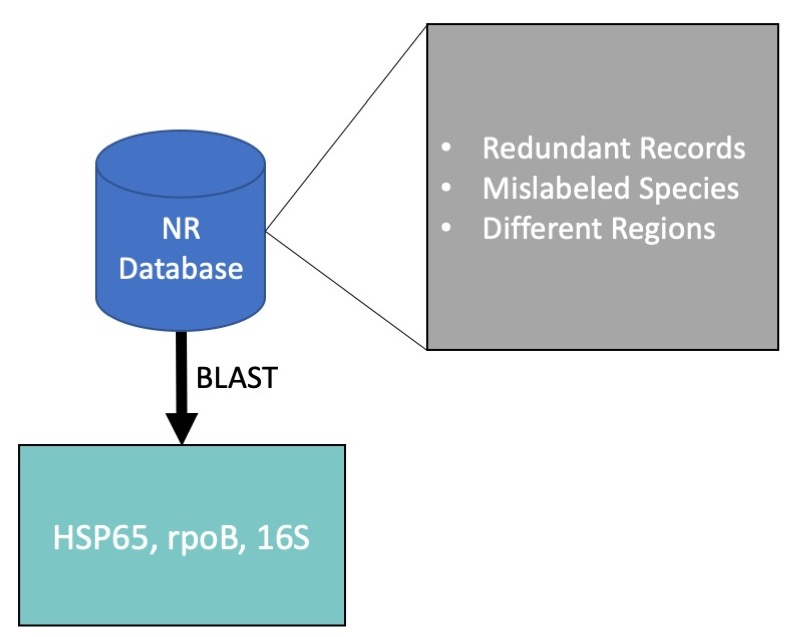
\includegraphics[height=5cm, width=5.5cm]{CPBS_11_18/Issues.jpg}
	\column{0.5\textwidth}
	\begin{block}{Redundant Records}
	Sequences between species are indistinguishable at gene
	\end{block}
	\begin{block}{Mislabeled Species}
	Naming conventions are constantly updated
	\end{block}
	\begin{block}{Different Regions}
	Current protocols amplify specific region of gene
	\end{block}
	\end{columns}
	
	%\tiny{Sczyrba, A., et al. Nature Methods 2017}
	\end{frame}
	%-----------------------------------------------------------
  \begin{frame}{Curated Gene Databases}
  \begin{block}{Number of Sequences per Species}
  The maximum number of sequences per species in the database is two
  \end{block}
  \center
  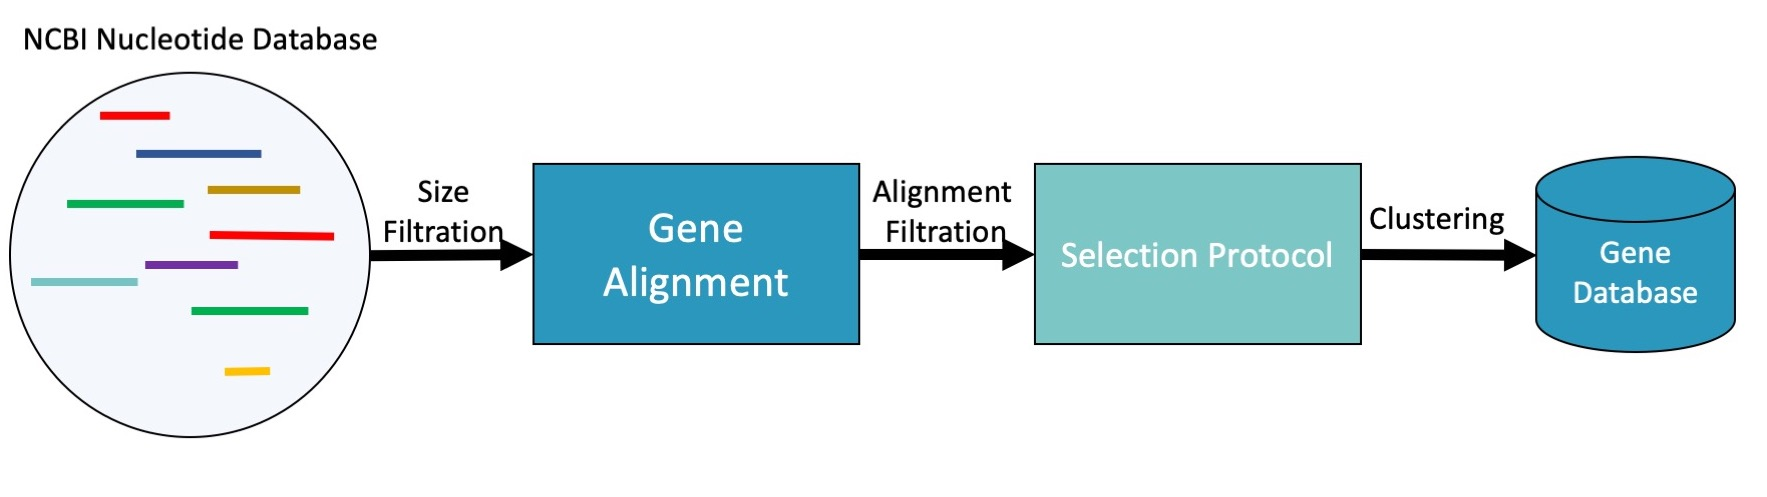
\includegraphics[height=4cm, width=11cm]{CPBS_11_18/Gene_Database_Workflow.jpg}
  \end{frame}


%-----------------------------------------------------------
  \begin{frame}{Selection Protocol}
  \center
  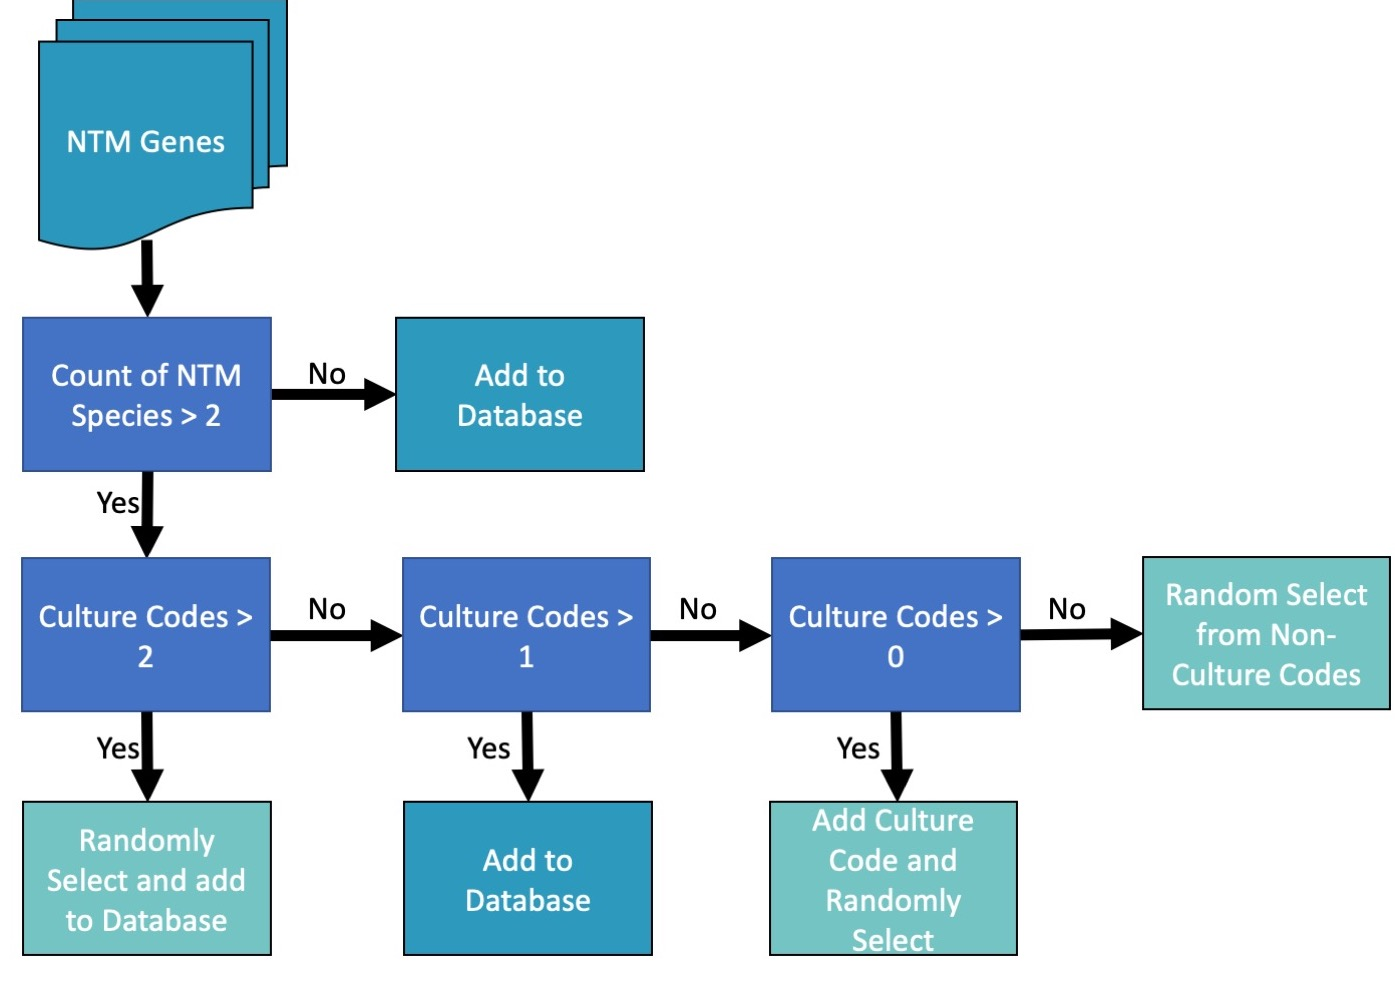
\includegraphics[height=7cm, width=11cm]{CPBS_11_18/Selection_Protocol.jpg}
  \end{frame}
%-----------------------------------------------------------
  \begin{frame}{Clinical Gene Databases}
  \begin{columns}
  \column{.3\textwidth}
  \begin{block}{hsp65}
  \begin{itemize}
  \item 382 base region  
  \item 185 species
  \end{itemize}
  \end{block}
  
  
  \column{.3\textwidth}
  \begin{block}{rpoB}
  \begin{itemize}
  \item 657 base region
  \item 134 species
  \end{itemize}
  \end{block}
  
  \column{.35\textwidth}
  \begin{block}{16S}
  \begin{itemize}
  \item 1470 base region
  \item 184 species
  \end{itemize}
  \end{block}

  \end{columns}
  \begin{block}{Species Overlap}
  107 species overlap between all three databases
  \end{block}
  
  \end{frame}
%-----------------------------------------------------------
	
	

	%-----------------------------------------------------------
	\begin{frame}{Database Availability}
	\begin{columns}
		\column{.5\textwidth}
			\begin{block}{Virus - 0.12 Mb}
			\begin{itemize}
			\item Bacillus phage Pony
			\item Caulobacter phage CcrColossus
			\item Mycobacterium phage Bxb1
			\item Mycobacterium phage Che9d
			\item Mycobacterium phage TM4
			\item Pseudomonas phage vB-PaeM-C2-10-Ab1
			\item Staphylococcus phage CNPH82
			\item uncultured phage crAssphage
			\end{itemize}
			\end{block}	
		\column{.6\textwidth}
			\begin{block}{Bacteria - 4.72 Mb}
			\begin{itemize}
			\item Bacillus subtilis subs. subtilis 168
			\item Clostridium acetobutylicum ATCC 824
			\item Clostridium perfringes str. 13
			\item Lactococcus lactis subsp. lactis Il1403
			\item Pseudomonas aeruginosa LESB58
			\item Staphylococcus aureus subsp. aureus N315
			\item Streptococcus pyogenes M1 476
			\item Xylella fastidiosa 9a5c
			\end{itemize}
			\end{block}
	\end{columns}
	\end{frame}
	%-----------------------------------------------------------
	\begin{frame}{Tools Used in Study}
	\begin{block}{Assembler}
	MEGAHIT - Effective at assembling viromes \\
	\tiny{Roux, S, et al. PeerJ 2017}
	\end{block}
	
	\begin{block}{Viral Contig Identification Methods}
	VirFinder - Viral contig K-mer identification model \\ 
	\tiny{Ren, Jie, et al. Microbiome 2017}
	
	\large{Blastx - Filtering against a viral protein database} \\
	\tiny{Camacho C., et al. BMC Bioinformatics 2008} \\
	
	\large{VirSorter - Hybrid HMM and gene marker database} \\
	\tiny{Roux, S., et al. PeerJ 2015} \\
	
	\large{vHMM - Iterative HMM trained on viral genes} \\
	\tiny{Paez-Espino, D., et al. Nature 2016} 
	
	\end{block}
	
	
	\end{frame}
	
%-----------------------------------------------------------
	\begin{frame}{Conclusions and Future Directions}
	
	\begin{block}{Performance}
	  The variance of tool performance suggests that no single tool is optimal for viral filtration
	\end{block}
	
	
	\begin{block}{Tool Parameter Optimization}
	Used default tool parameters for all tools
	\begin{itemize}
	\item Lenient BLASTX filtering resulting in false positives
	\item vHMM model is the second iteration
	\end{itemize}
	\end{block}
	
  \end{frame}
	
%-----------------------------------------------------------

\section{Duobiome}
\subsection{}

	
	\begin{frame}{Microbiome}
	\begin{columns}
	\column{0.5\textwidth}
	\begin{block}{Difficulties of phage study}
	\begin{itemize}
		\item Lack of universal marker gene
		\item Sequence heterogeneity 
		\item Misclassification in databases
	\end{itemize}
	\end{block}
		
		
	\begin{block}{Phage Isolation Methods}
	\begin{itemize}
		\item Biological filtration
		\item In silico methods
	\end{itemize}
	\end{block}
	
	\column{0.5\textwidth}
	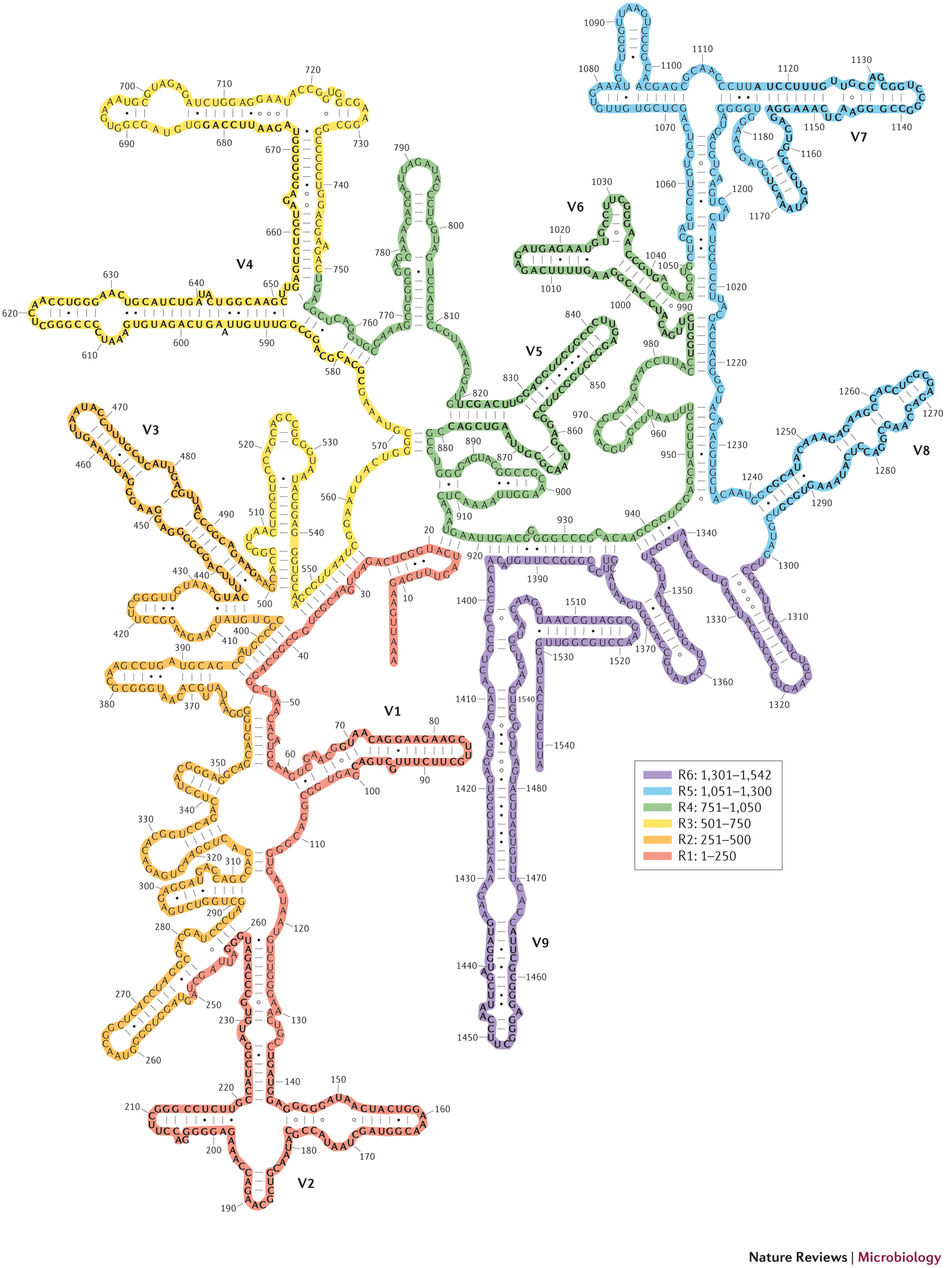
\includegraphics[height=5.5cm, width=5cm]{ribosome.jpg} \\
	\tiny{Yarza, P., et al. Nature Reviews Microbiology 2014}
	\end{columns}
		
	
	\end{frame}
	%-----------------------------------------------------------
	\begin{frame}{Degenerate Primers}
	\begin{block}{Current Methods}
	\begin{itemize}
	\item NCBI Webserver
	\item ESearch / Efetch function
	\item biomartr R package
	\end{itemize}
	\end{block}
	
	\begin{block}{Test Case}
	Retrieve protein sequences of three Mycobacterium subspecies \\ 
	\begin{itemize}
	\item Mycobacterium avium paratuberculosis
	\item Mycobacterium abscessus massiliense
	\item Mycobacterium abscessus bolletii
	\end{itemize}
	\end{block}
	
	\end{frame}
	%-----------------------------------------------------------
	
	\begin{frame}{Analyze both}
	\begin{block}{Batch Download Process}
	\begin{itemize}
	\item Query Assembly: "Mycobacterium abscessus \alert{subsp.} massiliense"[Organism] OR "Mycobacterium abscessus \alert{subsp.} bolletii"[Organism] OR "Mycobacterium avium \alert{subsp.} paratuberculosis"[Organism] 
	\item Select Complete Genome Tab
	\item Click "Download Assemblies" button and select Protein FASTA from File Type drop down 
	\end{itemize}
	\end{block}
	\begin{block}{Difficulties}
	\begin{itemize}
	\item Query string must to be specific
	\item Length of query string can become unwieldy
	\item Sparse information on download procedure and examples
	\end{itemize}
	\end{block}
	\end{frame}
	%-----------------------------------------------------------
	
	
	\begin{frame}{Testing against BLAST based and tradtional pipeline}
	
	\begin{block}{Efetch Retrieval Process}
	Efetch can be utilized via Python or via command-line
	
	\texttt{handle = Entrez.efetch(db="nuccore", id= \alert{UID\_List} , rettype = "fasta\_cds\_aa")}
	
	\end{block}
	
	\begin{block}{biomartr Sequence Retrieval}
	\texttt{library(biomartr) \\
	meta.retrieval(kingdom = "bacteria", \alert{group = "Actinobacteria"}, db = "genbank", type = "proteome")}
	\end{block}
	
	\begin{block}{Difficulties}
	\begin{itemize}
	\item Entrez.efetch function requires \textit{a priori} knowledge of Entrez UID 
	\item biomartr only able to bulk download phylum level
	\item Programming skills important [not required for Efetch]
	\end{itemize}
	\end{block}
	
	\end{frame}
	%-----------------------------------------------------------
	
	
	\begin{frame}{Genomic Retrieval and Blast Database Creation}
	\center
	GRAB Pipeline
	
	
	\end{frame}
	%-----------------------------------------------------------
	\begin{frame}{Future Directions}
	\begin{block}{Webserver}
	Shiny web application in development
	\end{block}
	
	\begin{block}{Viral GRAB}
	\begin{itemize}
	\item Expansion of GRAB to viral elements
	\item Features include ability to filter viruses by genetic material type
	\end{itemize}
	\end{block}
	\end{frame}
	
	

\section{Virulence Factors in Bacteriophages}
\subsection{}
	
	\begin{frame}{Endogenous Viral Elements (Prophages)}
	\begin{block}{Lysogenic Life Cycle}
	Viruses can integrate into host for an extended period of time
	\center
	\vspace{-0.2cm}
	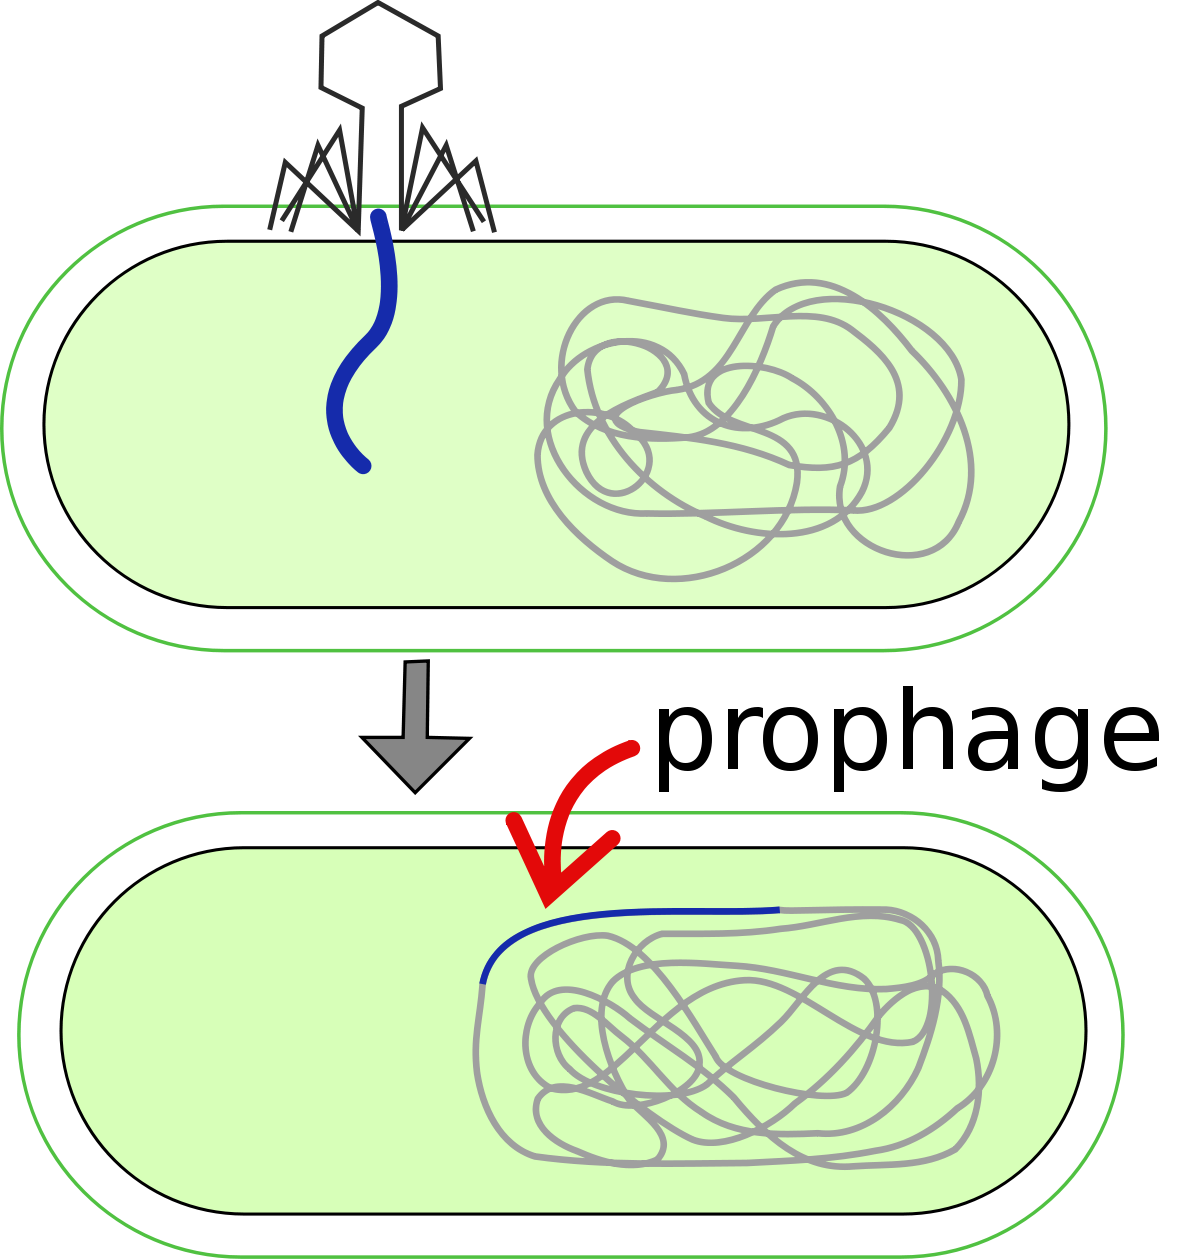
\includegraphics[height=3.5cm, width=5cm]{prophage.png}
	\end{block}
	\begin{block}{Importance of Prophages}
	Prophages can confer advantages to host improving survival \\ 
	Prophages are important to the emergence of pathogenic bacteria
	\end{block}
	
	\tiny{Canchaya C., et al. Curr Opin Microbiol 2003 \\ Wagner PL. \& Waldor MK. Infect Immune 2002}
	\end{frame}

	\begin{frame}{Finding Prophages}
	\begin{block}{Prophage Discovery Problem}
	Same difficulties as gene prediction: finding signal in data
	\center
	
\includegraphics[height=4cm, width=5cm]{dna.png}
	\end{block}
	\end{frame}
	
	\begin{frame}{Prophage Discovery Tools}
	\begin{block}{Number of Tools}
	10 tools listed at Omic Tools for prophage discovery
	\end{block}
	\begin{block}{Methods Used}
	\begin{itemize}
	\begin{columns}
	\column{0.5\textwidth}
	\item Sequence similarity
	\item Hidden Markov models 
	\item Transcription direction
	\column{0.5\textwidth}
	\item Protein length
	\item Sliding window GC content
	\item Phage specific kmer
	\end{columns}
	\end{itemize}
	\center
	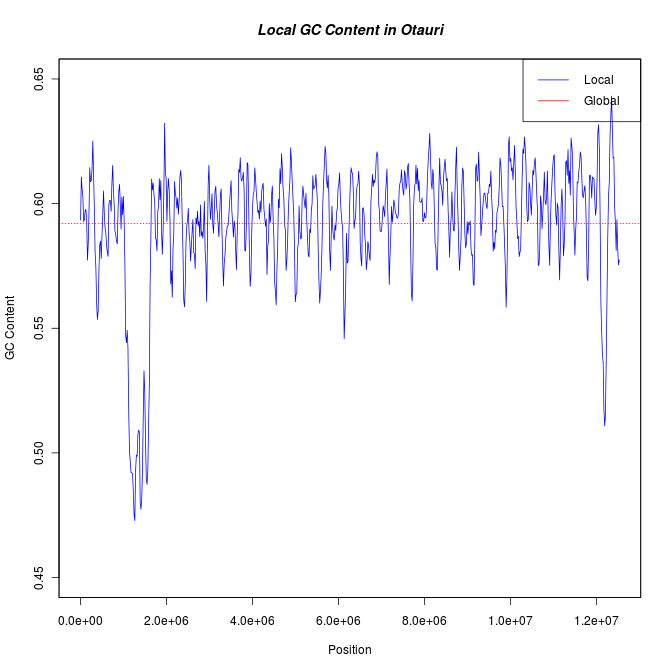
\includegraphics[height=3.5cm, width=5cm]{gc.png}
	\end{block}
	\end{frame}
	
	\begin{frame}{Prophage Discovery Methods}
	\begin{block}{Top Down Methods}
	All prophage discovery methods find prophages within contiguous sequences or genomes
	\center
	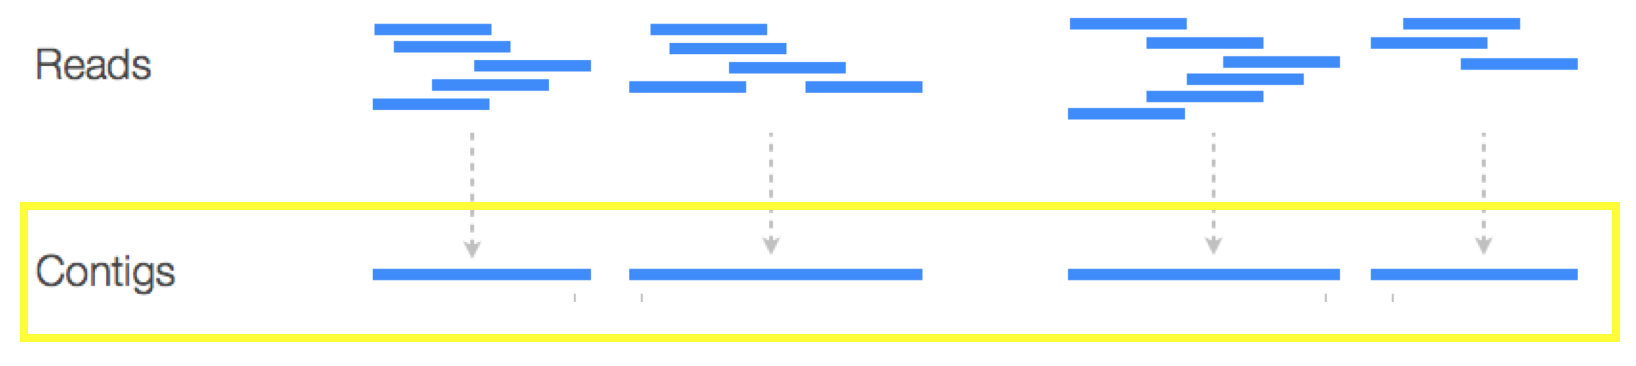
\includegraphics[height=3cm, width=5cm]{box_contigs.png}
	\end{block}
	
	
	\begin{block}{Potential Prophage Tool Pitfalls}
	\begin{itemize}
	\item Metagenomics produces short contigs that are discarded
	\item In metagenomics, prophage hosts may not be identified 
	\end{itemize}
	\end{block}
	
	
	\end{frame}
	

	
	\begin{frame}{Building Up Domains (BUD) Algorithm}
	\begin{block}{Initialization}
	\begin{itemize}
	\item Metagenomic reads are filtered by BLAST against Viral RefSeq
	\item Remaining reads are assembled into contigs
	\end{itemize}
	\end{block}
	\vspace{-0.5cm}
	\center
	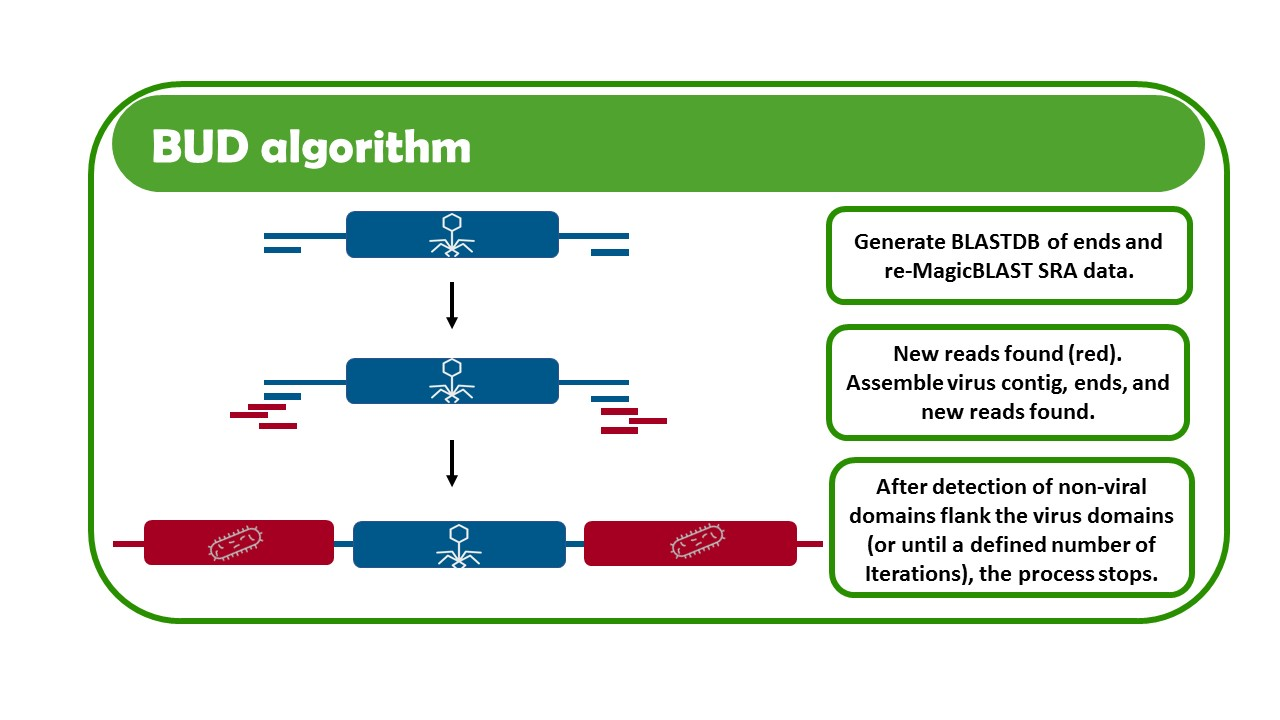
\includegraphics[height=6.75cm, width=10cm]{BUD_Algorithm.jpg}
	
	\end{frame}
	
	\begin{frame}{Potential Uses of BUD	}

	\begin{block}{Expanding Known Phage Host Range}
	BUD has the potential to identify novel hosts for prophages
	
	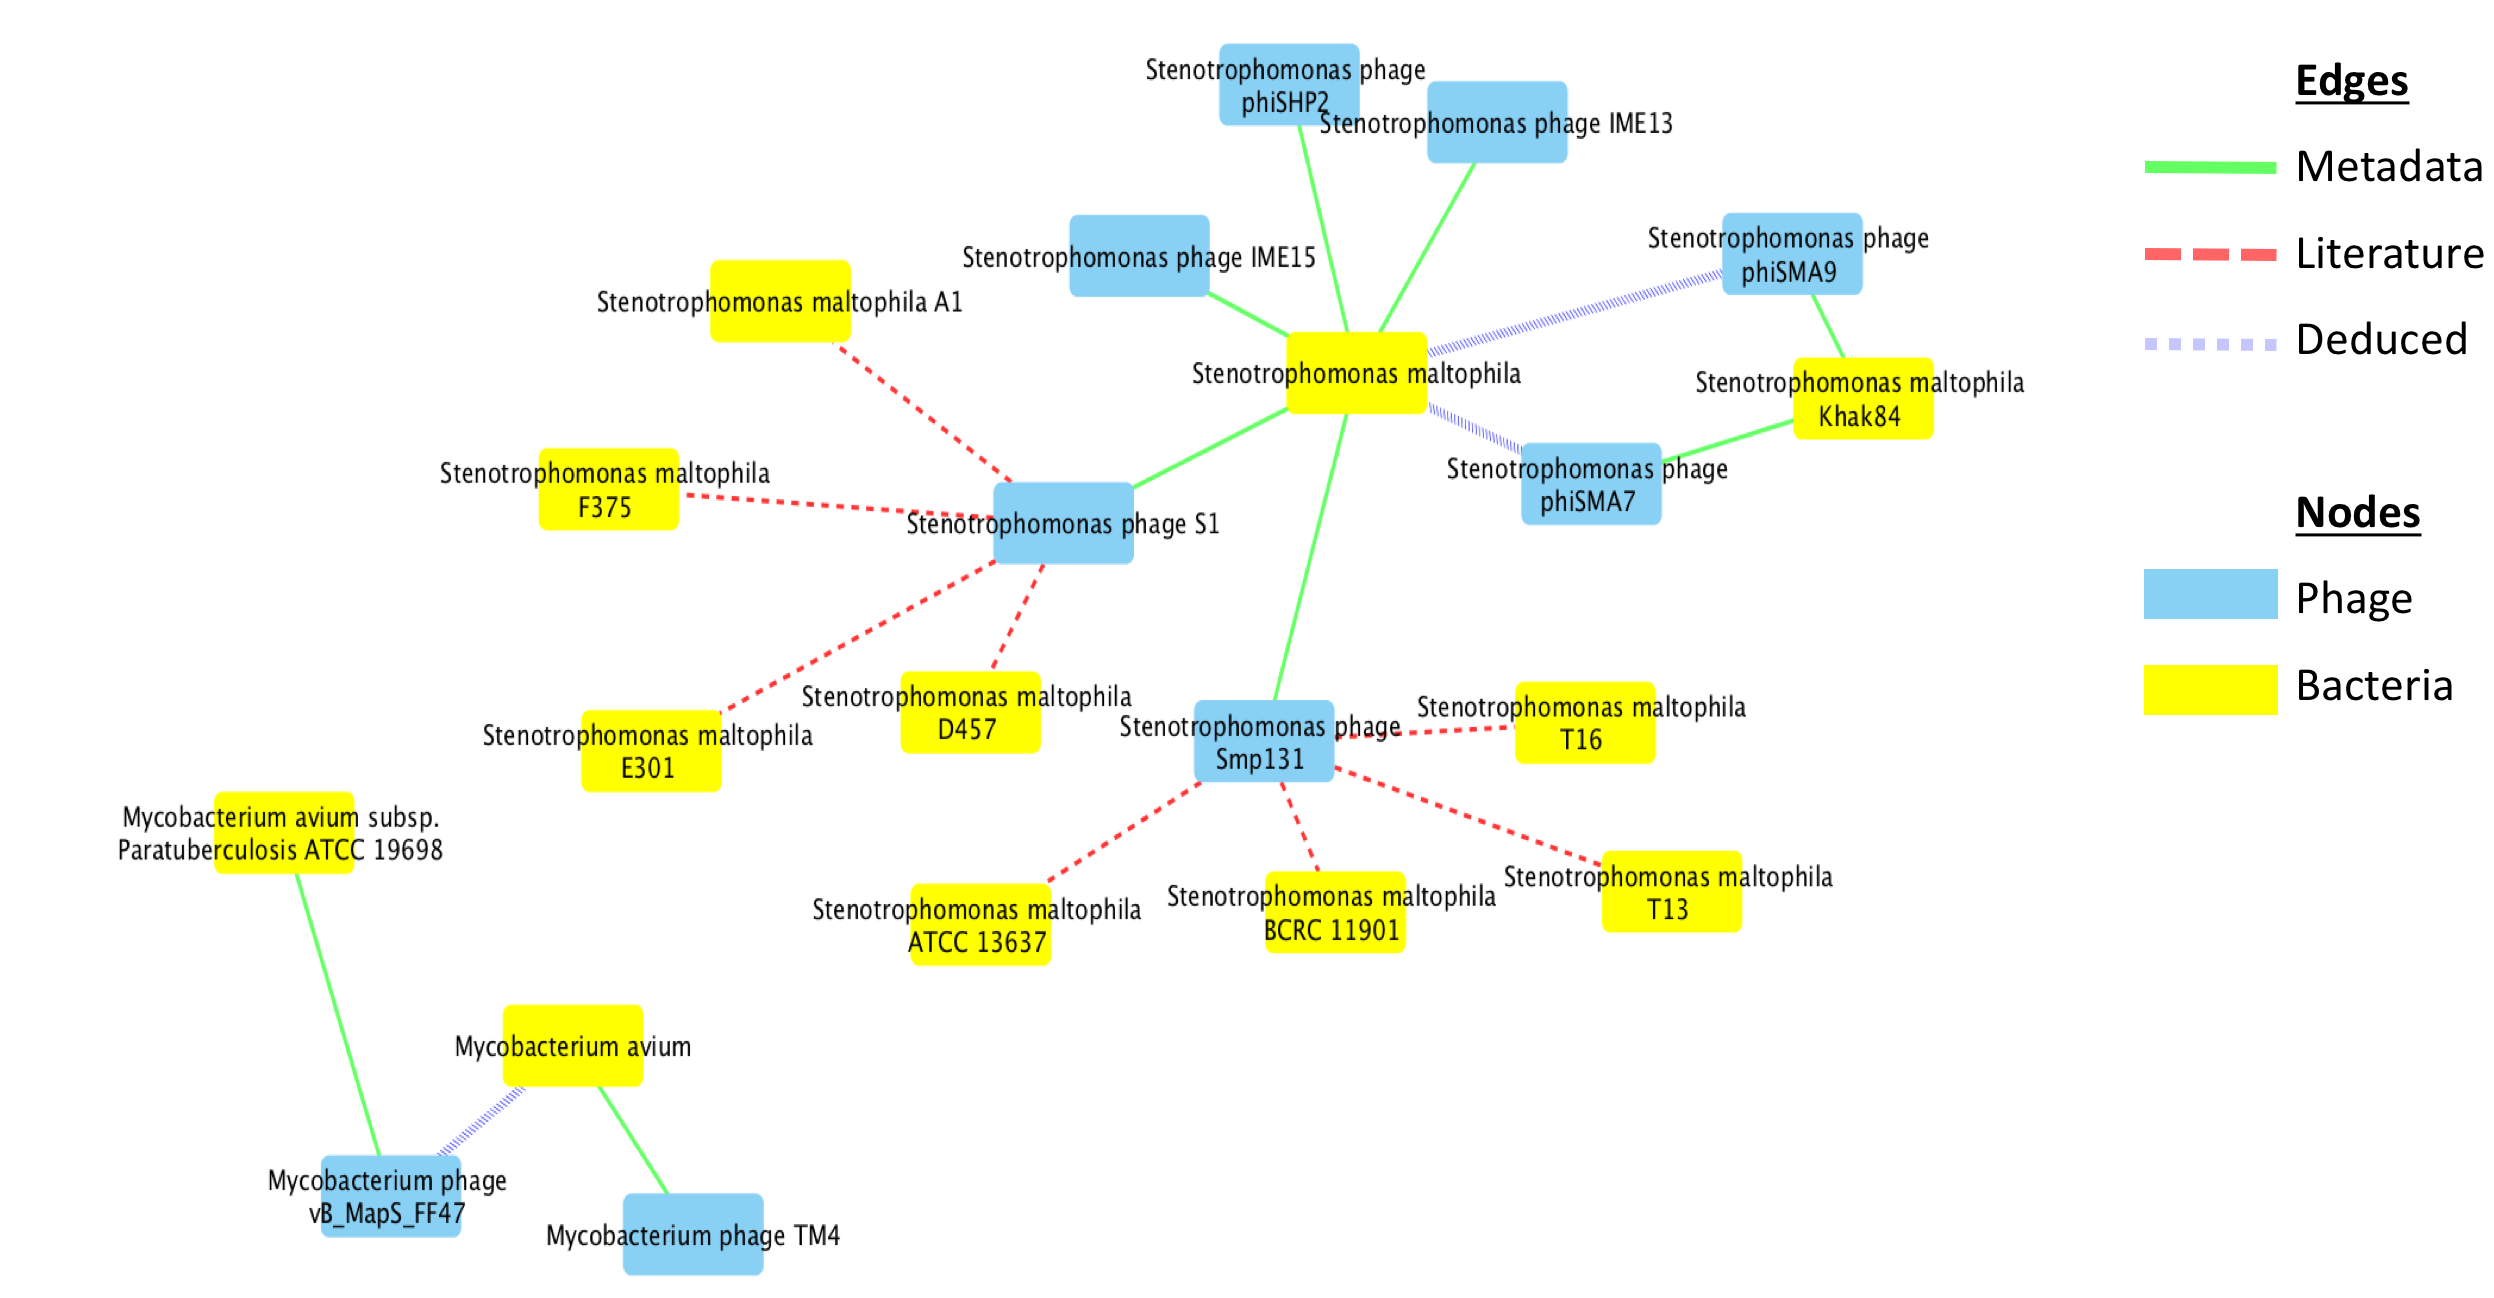
\includegraphics[height=6cm, width=11cm]{network.png}
	\end{block}
	
	\end{frame}
	
	\begin{frame}{Current Implementations of BUD}
	\begin{block}{ViruSpy}
	\begin{itemize}
	\item Originally written for NCBI Hackathon
	\item BUD Algorithm written in Perl and BASH
	\item Utilized Magic-BLAST for streaming of reads 
	\end{itemize}
	\end{block}
	
	\begin{block}{EndoVir}
	NCBI Collaborators Jan Buchman and Ben Busby \\ 
	\begin{itemize}
	\item Written in Python
	\item Implementation of BUD with Magic-BLAST
	\end{itemize}
	\end{block}
	\end{frame}
	
	\begin{frame}{Future Directions}
	\begin{block}{Magic-BLAST Streaming}
	Create a version of BUD for local metagenomic sequences 
	\end{block}
	
	\begin{block}{Testing Performance of BUD}
	Using the simulated dataset from previous study to compare the performance of identifying prophages by current tools against BUD
	\center
	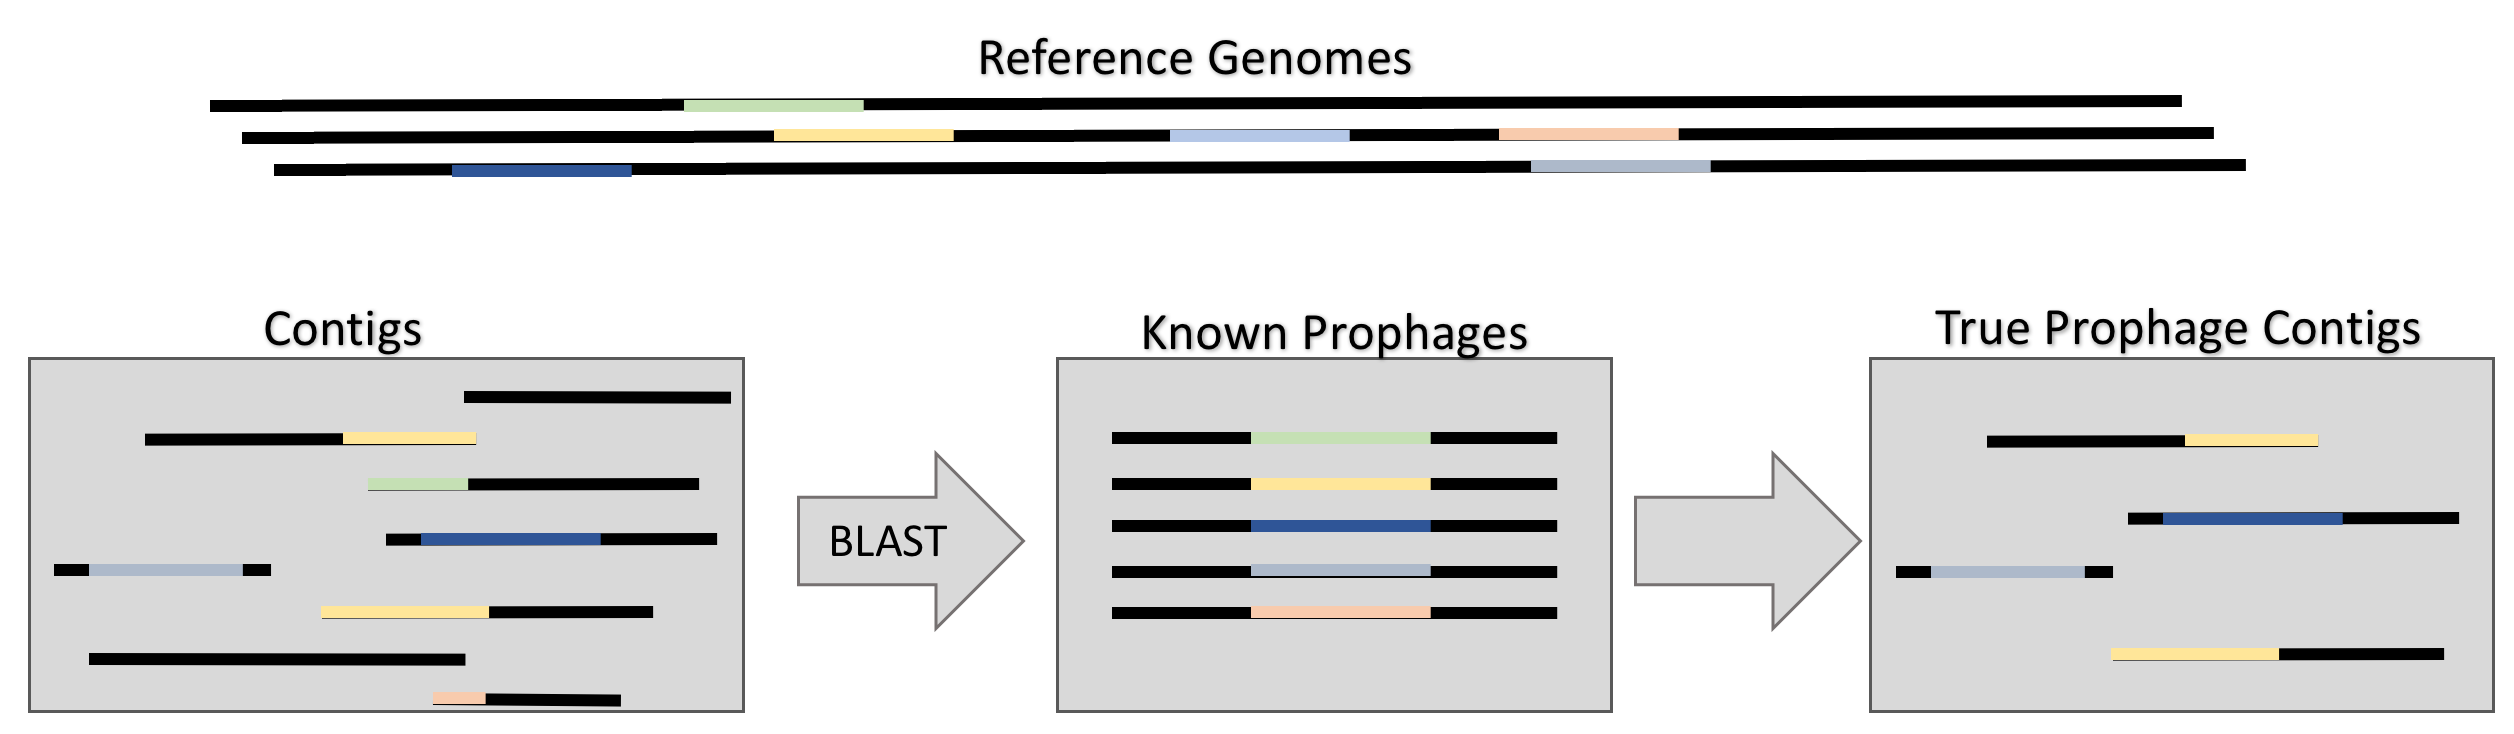
\includegraphics[height=4cm, width=8cm]{fig.png}
	
	\end{block}
	\end{frame}
	
	
\section{Hybrid Viral Contig Prediction}
\subsection{}
	\begin{frame}{Building Up Domains (BUD) Algorithm}
	\begin{block}{Initialization}
	\begin{itemize}
	\item Metagenomic reads are filtered by BLAST against Viral RefSeq
	\item Remaining reads are assembled into contigs
	\end{itemize}
	\end{block}
	\vspace{-0.5cm}
	\center
	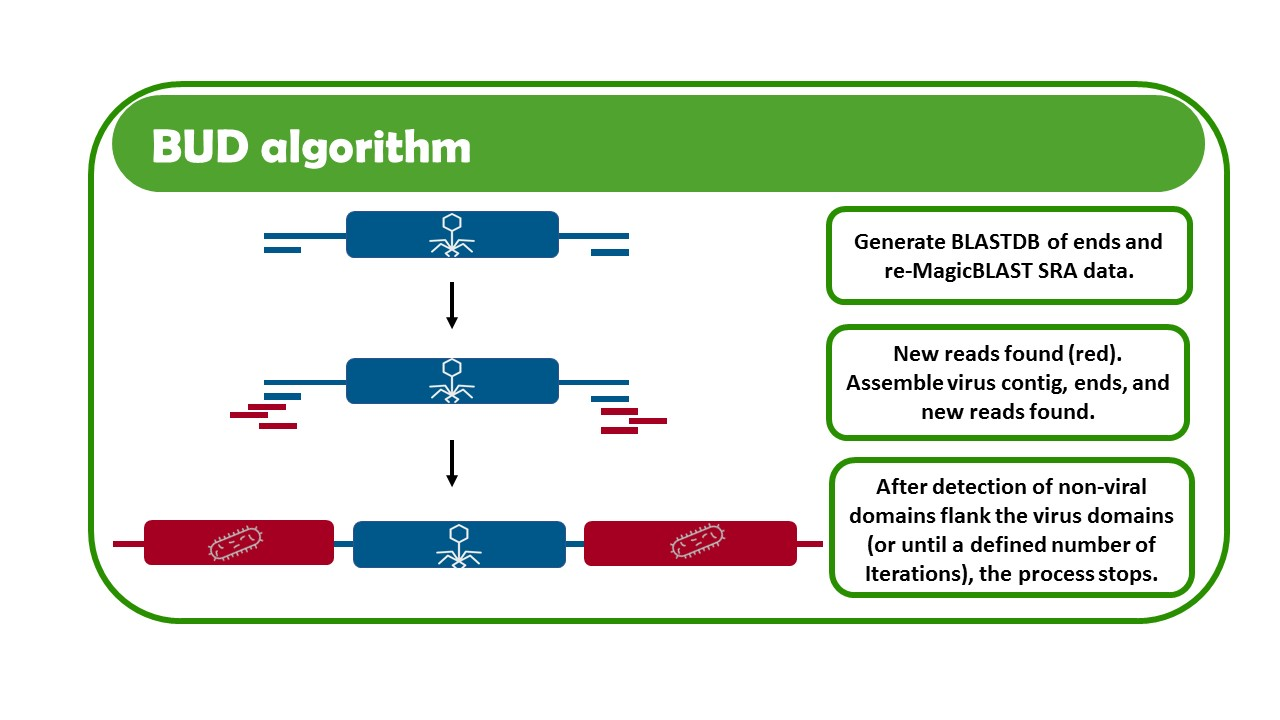
\includegraphics[height=6.75cm, width=10cm]{BUD_Algorithm.jpg}
	
	\end{frame}
	


\section{}

	\begin{frame}{Concluding Remarks}
	\center
	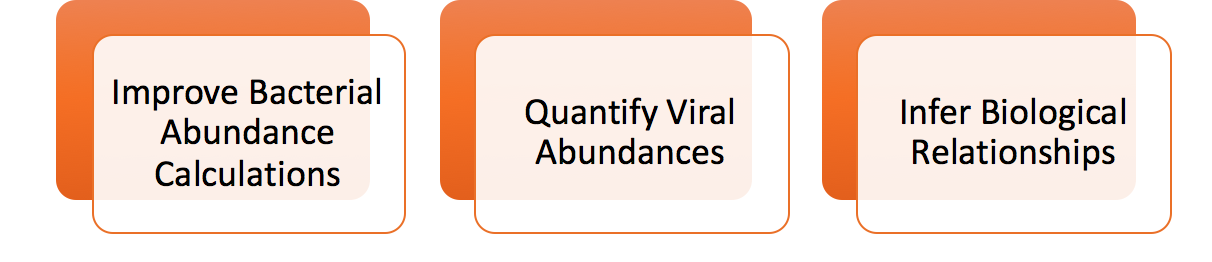
\includegraphics[height=2cm, width=10cm]{goals.png}
	\begin{columns}
	\column{0.3\textwidth}
	\begin{block}{Metagenomic Simulation Study}
	Effectively identifying viral elements improves bacterial abundance calculation
	\end{block}
	\column{0.3\textwidth}
	\begin{block}{GRAB}
	Viral GRAB will contribute to a focus on phages specific to lung infections
	\end{block}
	\column{0.3\textwidth}
	\begin{block}{Building Up Domains}
	Allows for the identification of prophages elements in metagenomics
	\end{block}
	
	\end{columns}
	
	\end{frame}
	
	
	
	
	\begin{frame}{}
	\vspace{1cm}
	{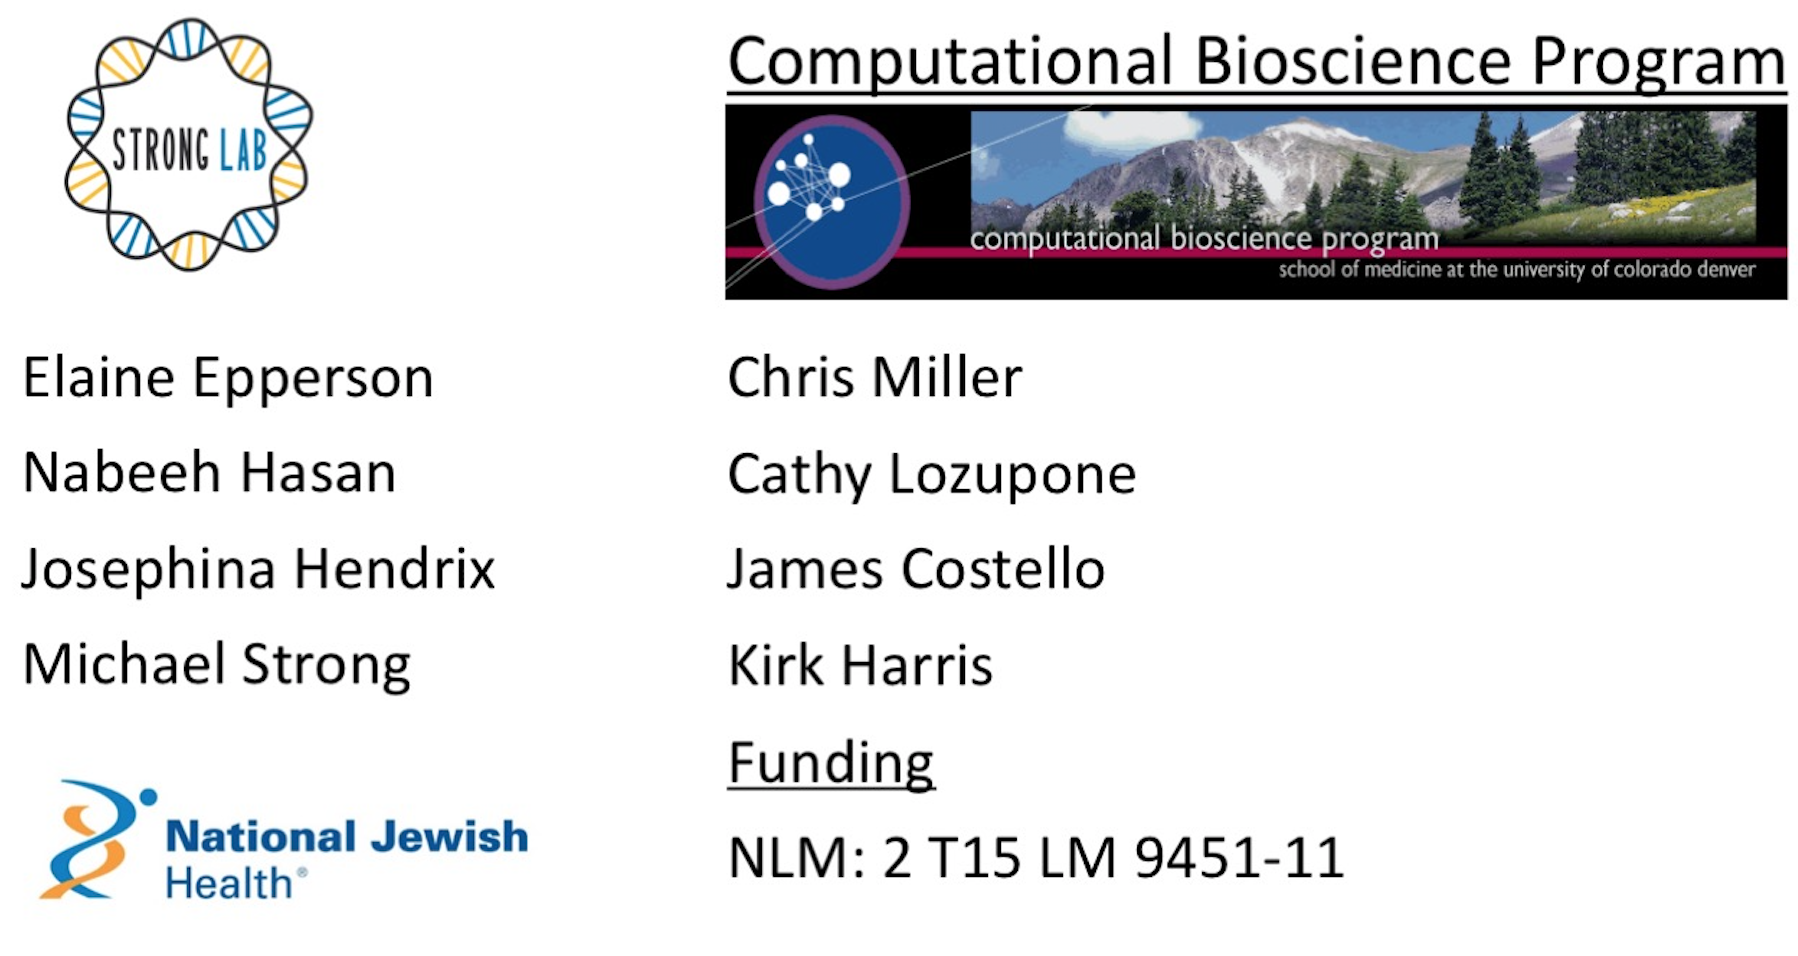
\includegraphics[height=8cm, width=11cm]{Acknowledgements.png} }
	\end{frame}
	
	
	\begin{frame}{Questions?}
	\center
	Cody Glickman \\ 
\includegraphics[height=2cm, width=2cm]{lablogo.png} \\ cody.glickman@ucdenver.edu \\ \alert{www.github.com/glickmac} \\ www.codyglickman.com
	\end{frame}
	
	
	\begin{frame}{Bias in Average Fold Coverage by GC}
	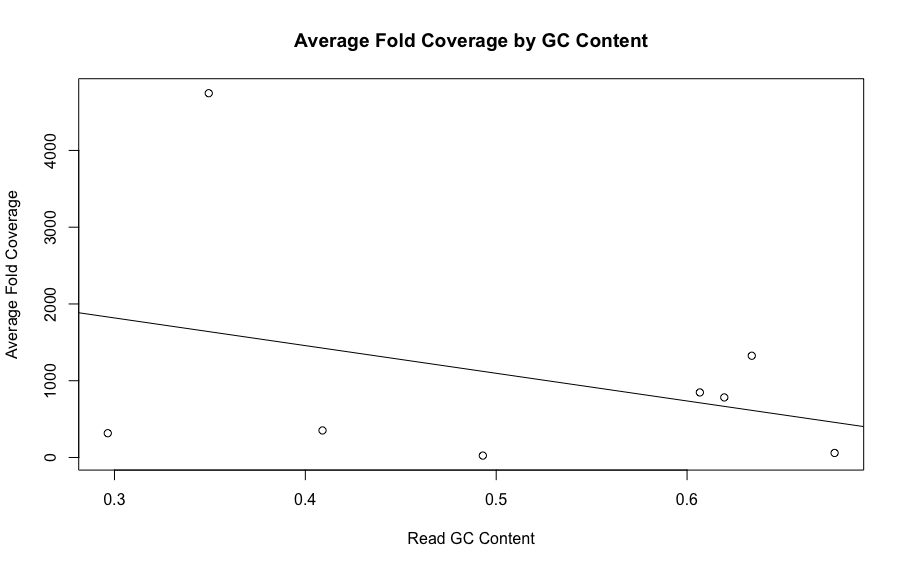
\includegraphics[height=8cm, width=11cm]{Viral_Coverage_by_GC.png}
	\end{frame}
	
	
	\begin{frame}{My Pipeline}
	\vspace{-1cm}
	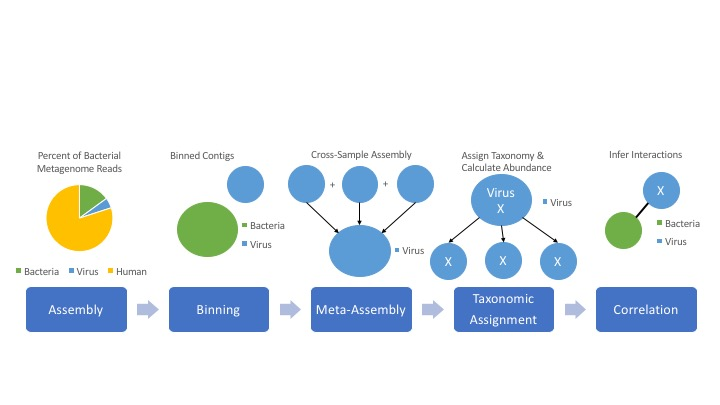
\includegraphics[height=6cm, width=11cm]{figure_2_updated.jpg}
	\end{frame}
	
	
	\begin{frame}{Tools Used in Study Continued}
	\begin{block}{Simulation Tools}
	BBMAP - a suite of tools designed for sequencing data \\
	\tiny{Bushnell, B., JGI 2016}
	\end{block}
	
	\begin{block}{Taxonomic Identification}
	Kraken - A reference-free K-mer taxonomic identifier \\
	\tiny{Wood, Derrick E., and Steven L. Salzberg Genome 2014}
	
	\large{Blastx - Referenced against a viral protein database} \\
	\tiny{Camacho C., et al. BMC Bioinformatics 2008}
	\end{block}
	
	\begin{block}{Prophage Identification}
	Phaster - A popular prophage discovery web tool  \\
	\tiny{Arndt, David, et al., Nucleic Acids Research 2016}
	\end{block}
	\end{frame}
	
	%\begin{itemize}
	%\item Prophages in bacterial reference genomes are well annotated
	%\item Location in bacterial reference genome is well annotated
	%\item find prophages in contigs and map contigs to reference.
	
	
\end{document}